\lecture{3}{17 Sep. 13:20}{}
\begin{prev}
    \(G = (G, *)\) is called a group if 
    \begin{itemize}
        \item [(1)] \((a * b) * c = a * (b * c)\)
        \item [(2)] \(\exists e \in G\) s.t. \(a * e = a = e * a\). 
        \item [(3)] For \(a \in G\), \(\exists a^{-1} \in G \) s.t. \(a * a^{-1} = e = a^{-1} * a\).      
    \end{itemize} 
    Also, we have shown that \(e\) is unique and for every \(a \in G\), \(a^{-1} \) is also unique.   
\end{prev}

\begin{definition}[Subgroup] \label{def: subgroup}
    Suppose \(G = (G, *)\) is a group, and \(H \subseteq G\), then \(H\) is called a subgroup if \((H, *)\) is a group.   
\end{definition}

\begin{figure}[H]
    \centering
    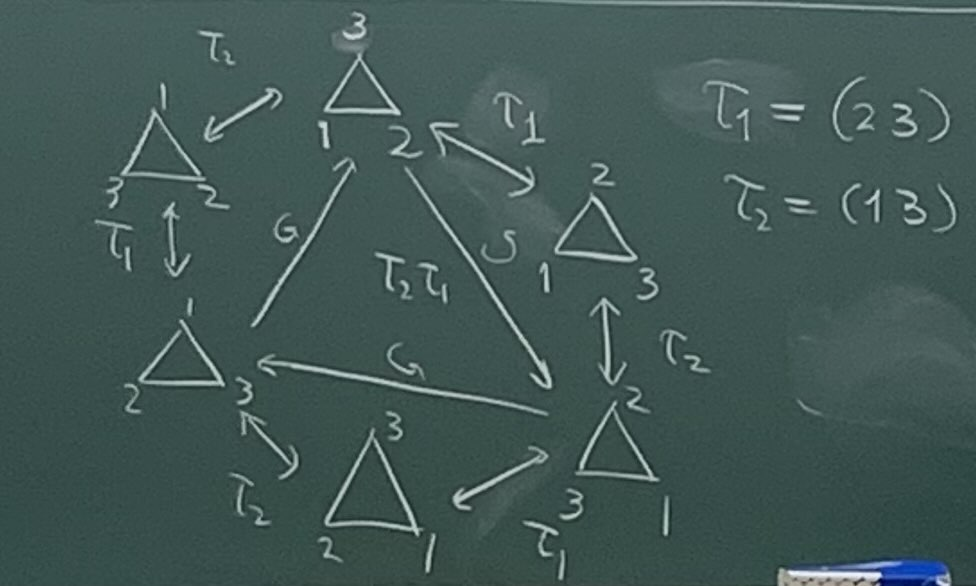
\includegraphics[width=0.6\textwidth]{./Figures/IMG_3952.jpg}
    \caption{Traingle groups}
    \label{fig:triangle groups}
\end{figure}
\begin{eg}
    Consider the case when 
 \[
    G = \left\{ \text{permutations on } \left\{ 1,2,3 \right\}  \right\} = \mathcal{S} _3, 
 \] then what is the subgroup of \(G\)? 
\end{eg}
\begin{explanation}
    Note that 
    \[
        G = \left\{ id, \tau _1, \tau _2, \tau _1 \tau _2 \tau _1, \tau _1 \tau _2, \tau _2, \tau _1 \right\}. 
    \]
    Then, 
    \begin{align*}
        H &= \left\{ id \right\}, \left\{ id, \tau _1 \right\}, \left\{ id, \tau _2 \right\}, \left\{ id, \tau _1 \tau _2 \tau _1 \right\}, \\
        &\quad \, \left\{ id, \tau _1 \tau _2, \tau _2 \tau _1 \right\}, G     
    \end{align*}
    These \(6\) subgroups are all subgroups of \(G\). In general, identity \(\left\{ id \right\} \) and \(G\) itself are always subgroups.    
\end{explanation}

\begin{note}
    We will talk about Sylow's theorem later, which claims that if
    \[
        \vert G \vert = p_1^{e_1} \dots p_r^{e_r},
    \] then \(G\) has subgroups of order \(p_i^{e_i}\) for \(1 \le i \le r\).  
\end{note}

\begin{eg}
    If \(G=(\mathbb{Z} , +)\), what is the subgroup of \(G\)?
\end{eg}
\begin{explanation}
    Suppose \(n \in H\), then \(n + n = 2n \in H\), and \(-n \in H\), and then \(3n = 2n + n \in H \). Hence, all multiples of \(n \in H\), which means \(n \mathbb{Z} \subseteq H\). If \(n_1, \dots , n_r \in H\), then 
    \[
        \underbrace{n_1 \mathbb{Z} + n_2\mathbb{Z} + \dots + n_r\mathbb{Z}}_{d\mathbb{Z} } \subseteq H,
    \] where \(d = \gcd(n_1, n_2, \dots , n_r)\). Hence, the only subgroups are of the form \(d \mathbb{Z}\). In particular, \(0 \mathbb{Z} = \left\{ 0 \right\} \), which is the identity subgroup, and \(1 \mathbb{Z} = \mathbb{Z} \) is \(G\) itself.       
\end{explanation}

\begin{eg}
    If \(G = \mathbb{R} ^{\times } = (\mathbb{R} \setminus \left\{ 0 \right\}, \times  )\), what are the finite subgroups of \(G\)? 
\end{eg}
\begin{explanation}
    Consider \(H = \left\{ 1 \right\}, \left\{ 1, -1 \right\}  \), and these are all finite subgroups. 
\end{explanation}

\begin{eg}
    Suppose 
    \[
        G = \mathrm{GL}_n(\mathbb{R}) = \left( \left\{ n \times n \text{ invertible matrices} \right\}, \times \right),  
    \] then what are the subgroups?
\end{eg}
\begin{explanation}
    Consider 
    \[
        \mathrm{SL}_n(\mathbb{R} ) = \left\{ g \in \mathrm{GL}_n(\mathbb{R} ) \mid \det g = 1 \right\},  
    \] then since \(\det g \det h = \det (gh)\), so \(\mathrm{SL}_n(\mathbb{R} ) \) is a subgroup. Also, consider the set of all diagonal \(n \times n\) real matrices, then it is also a subgroup of \(\mathrm{GL}_n(\mathbb{R} ) \).    
\end{explanation}

\begin{remark}
    We define orthogonal subgroup to be the subgroup preserving distances. For example, suppose \(g \in \mathrm{GL}_n(\mathbb{R} ) \), and if we have norm here, then \(\vert gv \vert = \vert v \vert  \) if and only if \(g^t g = I\).  
\end{remark}

\begin{exercise}
    Show that 
    \[
        O_n(\mathbb{R} ) = \left\{ g \in \mathrm{GL}_n(\mathbb{R} ) \mid g^t g = I\right\} 
    \] forms a subgroup of \(\mathrm{GL}_n(\mathbb{R} ) \). 
\end{exercise}

